% BACKUP OF TIKZ PICTURES

\begin{figure}[htb] % (here, top, bottom, page)
  \centering
  % \def\svgwidth{\columnwidth}
  \input{images/pataphysicalisation.pdf_tex}
\caption[Pataphysicalisation]{Pataphysicalisation}
\label{fig:patasearch02}
\end{figure}

--------------------------------

\begin{figure}[htbp]
  \centering
  \begin{tikzpicture}
  [every node/.style={node distance=2cm},
  box/.style={rectangle, draw, fill=black!10, inner sep=5pt, text width=2cm, text badly centered, minimum height=1cm}]
  % Coordinate Grid for testing
  % \draw[gray,very thin] (0,0) grid (6,6);
  % \foreach \x in {0,1,2,3,4,5,6}
  % \draw (\x cm,1pt) -- (\x cm,-1pt) node[anchor=north] {$\x$};
  % \foreach \y in {0,1,2,3,4,5,6}
  % \draw (1pt,\y cm) -- (-1pt,\y cm) node[anchor=east] {$\y$};
  \node [box] (web) {Web};
  \node [box, below of=web] (crawl) {Crawler};
  \node [box, below of=crawl] (index) {Index};
  \node [box, right=1cm of index] (rank) {Ranking};
  \node [box, above of=rank] (query) {Query};
  \node [box, above of=query] (user) {User};
  \path[->,thick]
  (3.375,1) edge (user.north)
  (web) edge (crawl)
  (crawl) edge (index)
  (index) edge (rank)
  (query) edge (index)
  (user) edge (query);
  \draw [->] (rank.east) -| (5,0) -- (user.east);
  \end{tikzpicture}
  \caption[Search Engine Architecture]{Very abstract search engine architecture}
  \label{fig:SEA}
\end{figure}

------------------------------

% Definition of circles
\def\leftcircle{(0,0) circle (1.5cm)}
\def\rightcircle{(0:2cm) circle (1.5cm)}
\colorlet{circle edge}{black!50}
\colorlet{circle area}{black!20}
\tikzset{filled/.style={fill=circle area, draw=circle edge, thick},
    outline/.style={draw=circle edge, thick}}

\begin{figure}[htb]
  \centering
  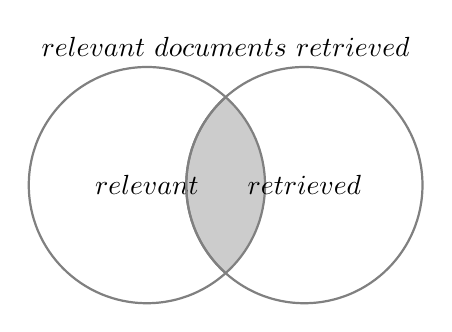
\begin{tikzpicture}
  \begin{scope}
  \clip \leftcircle;
  \fill[filled] \rightcircle;
  \end{scope}
  \draw[outline] \leftcircle node {$relevant$};
  \draw[outline] \rightcircle node {$retrieved$};
  \node[anchor=south] at (current bounding box.north) {$relevant \ documents \ retrieved$};
  \end{tikzpicture}
\caption[Precision and Recall]{Precision and Recall}
\label{fig:PR}
\end{figure}
